\chapter{数值模拟}

在过去的章节中,我们介绍了量子线路的基本概念,并介绍了如何使用基于Pauli路径积分的模拟算法来模拟量子线路。并在一些具体的线路模型中,研究了模拟算法的计算复杂度和误差。特别地,发现了在一些情况下,比如含噪声的变分量子线路,算法的计算复杂度关于线路规模是多项式关系。
虽然,我们定性地分析了模拟算法的计算复杂度,但是我们还没有给出具体的数值模拟结果。多项式复杂度对于实际的模拟算法来说是一个很好的性质,但是是否实用还有待进一步的数值模拟结果的验证。
例如,在定理~\ref{thm:main}中,我们得到了对于噪声\textbf{情况1}时,算法的计算复杂度是:
\begin{equation*}
    \mathrm{Poly}(n) \order{L} \bigg(\frac{\norm{O}_\infty}{\varepsilon \sqrt{\delta}} \bigg)^{\order{\frac{1}{\gamma}}},
\end{equation*}
其中$n$是线路的规模,$L$是线路的深度,$\varepsilon$是算法的精度,$\delta$是算法失败的概率,$\gamma=\min\{p|{p \in \{p_x,p_y,p_z\},p\neq 0}\}$是噪声率,$\norm{O}_\infty$是可观测量的无穷范数。当噪声强度$\gamma$很小时,例如$\gamma=0.01$,我们可以得到算法的计算复杂度是$\mathrm{Poly}(n) \order{L} \bigg(\frac{\norm{O}_\infty}{\varepsilon \sqrt{\delta}} \bigg)^{{100}}$,这是一个难以实现的计算复杂度。万幸的是,实际情况下的计算复杂度并不会达到这么高的程度,我们将在本章中具体说明。

除此之外,在这一章中,我们将使用基于Pauli路径积分的模拟算法来模拟一些量子线路的具体实例。并与实际的实验结果进行比较,以验证模拟算法的有效性。

在本章中,如未加说明,我们将假设环境噪声处于\textbf{情况1},这是因为在实际的量子计算机中,很难出现纯净的单独类型的Pauli错误。因此假设$p_x\neq 0,p_y\neq 0,p_z\neq 0$是合理的,此时与噪声关联的Hamming Weight 根据式~\eqref{eq:noise_hamming_weight}可以得到:
\begin{equation*}
    \abs{\bm{s}}_{\mathcal{N}}=\abs{\bm{s}}_X + \abs{\bm{s}}_Y + \abs{\bm{s}}_Z.
\end{equation*}
在这种情况下,正是原始的Hamming Weight定义,为了方便,我们将在本章中使用$\abs{\bm{s}}$来表示。


\section{模拟算法的计算复杂度}
对于变分量子线路,根据式~\eqref{eq:vqa:cost},在噪声\textbf{情况1}下,模拟算法的计算复杂度是:
\begin{equation*}
    \mathrm{Poly}(n) \order{L}2^M,
\end{equation*}
其中$n$是线路的规模,$L$是线路的深度,$M$是截断变量。可以看到在过去理论估计中,计算复杂度关于截断变量$M$是指数关系。这个指数因子的来源是由于在Pauli 路径枚举过程中,根据式~\eqref{eq:vqa:case1:N_M},符合条件$\abs{\bm{s}}\leq M$的Pauli路径数目是指数级别的。在这一节中,我们将通过具体的数值模拟结果来估计,给定截断变量$M$时,满足条件Pauli路径的真实数目。

在本节中,考虑的噪声模型均为退极化噪声模型,即满足$p_x=p_y=p_z=\frac{\lambda}{4}$,其中$\lambda$是噪声强度。


对于截断变量的取值,根据引理~\ref{lemma:MSE_l}的注释,我们可以得到
对于变分量子线路在退极化噪声下,如果式~\eqref{eq:E_cross_equals_0}成立,那么对任意的$\nu > 0$,只要截断参数$M$满足:
\begin{equation}\label{eq:depolarizing_M}
    M\geq\frac{1}{2\lambda}\ln{\frac{\norm{O}_\infty^2}{\nu}},
\end{equation}
其中$\lambda$是退极化噪声的强度,那么含噪声期望值模拟的均方误差满足:
\begin{equation}
    \mathbb{E}_{\bm{\theta}}\left[\left(\widetilde{\langle O\rangle}-\widehat{\langle O\rangle}\right)^2\right]\leq\nu.
\end{equation}
事实上,在实际计算中,$M$也并不需要取到这么大的值,我们将在本节中具体用数值说明。

\subsection{计算复杂度与截断变量$M$的关系}

因为截断Pauli路径模拟算法的计算复杂度主要来自于具有非平凡贡献的Pauli路径的数量,因此我们将通过计算具有非零贡献的Pauli路径的数量来估计模拟算法的计算复杂度。在这一节中,我们将通过具体的数值模拟结果来估计,给定截断变量$M$时,满足条件Pauli路径的真实数目。


\begin{figure}[htbp]
    \centering
    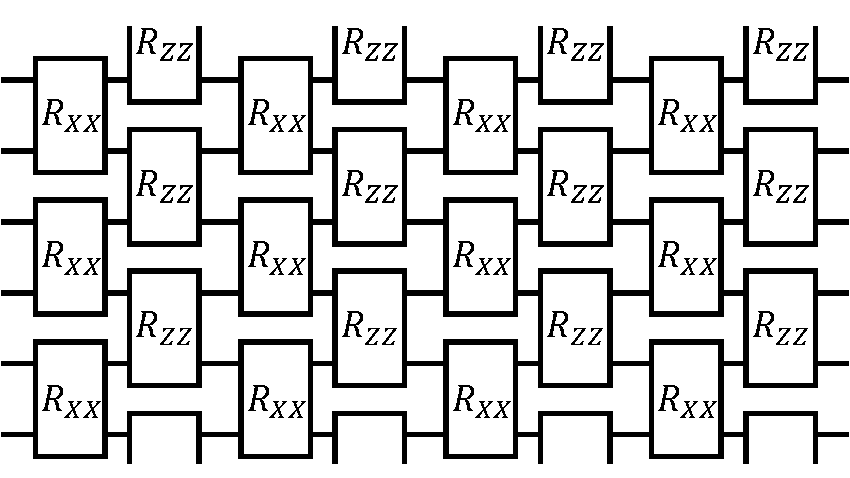
\includegraphics[width=0.5\textwidth]{figures/XX_ZZ_Ansatz.pdf}
    \caption{数值模拟计算复杂度与$M$的关系中使用的量子线路示意图}\label{fig:XX_ZZ_Ansatz}
\end{figure}

在我们的模拟中,我们考虑了一个具体的MaxCut问题实例。
对于给定的量子比特数$n$,我们随机生成一个$n\times n$的邻接$(0,1)$矩阵$A$,其中每个元素为$1$的概率为$0.5$。
可观测量$O$基于MaxCut问题构建,并按照给出的邻接矩阵$A$构造:
\begin{equation}
    O=\sum_{A_{i,j}=1} Z_iZ_j.
\end{equation}
在模拟中,初始状态的密度矩阵设为$\rho=\ketbra{0}{0}^{\otimes n}$。
考虑的量子线路$\mathcal{U}$如图~\ref{fig:XX_ZZ_Ansatz}所示,该线路由交替的$R_{XX}$和$R_{ZZ}$ 旋转门组成,其中第一个量子比特上的不完整$R_{ZZ}$门表示它们作用于第一个和最后一个量子比特。


\begin{figure}[hbp]
    \centering
    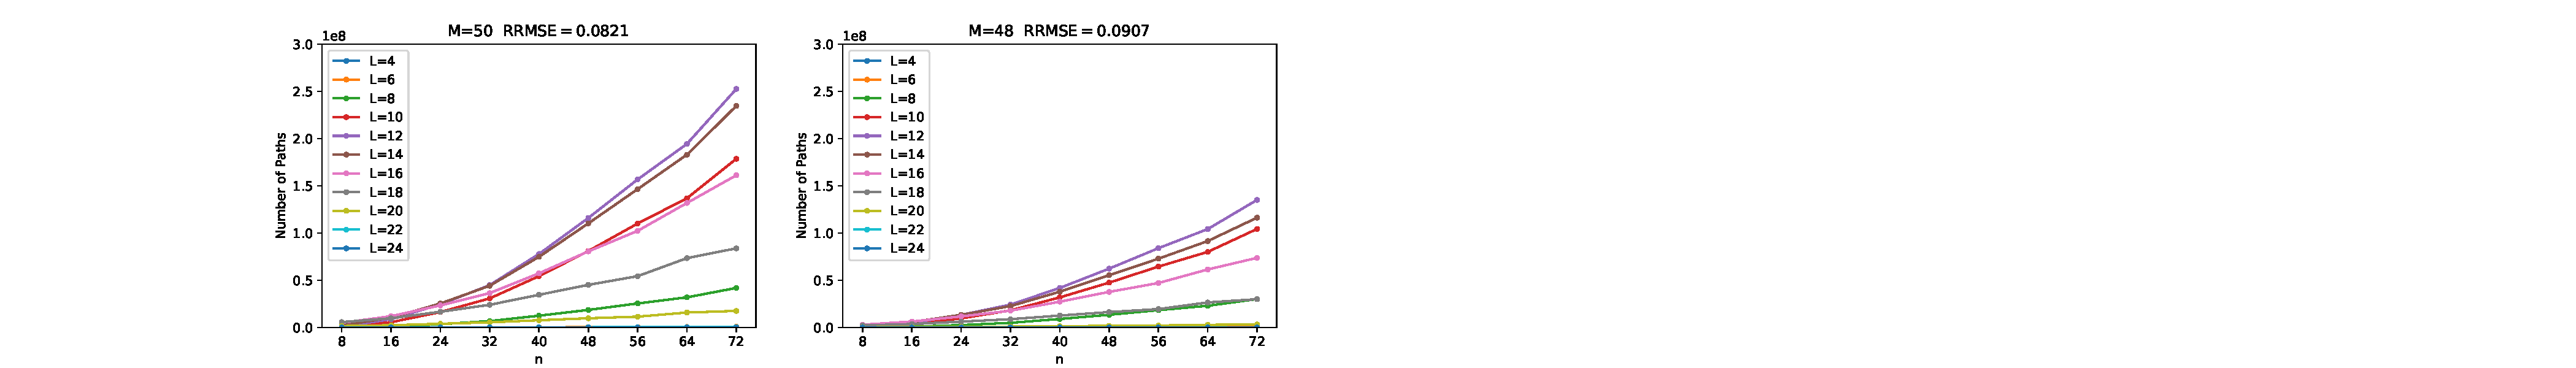
\includegraphics[width=\textwidth]{figures/depth_path2_p1}
    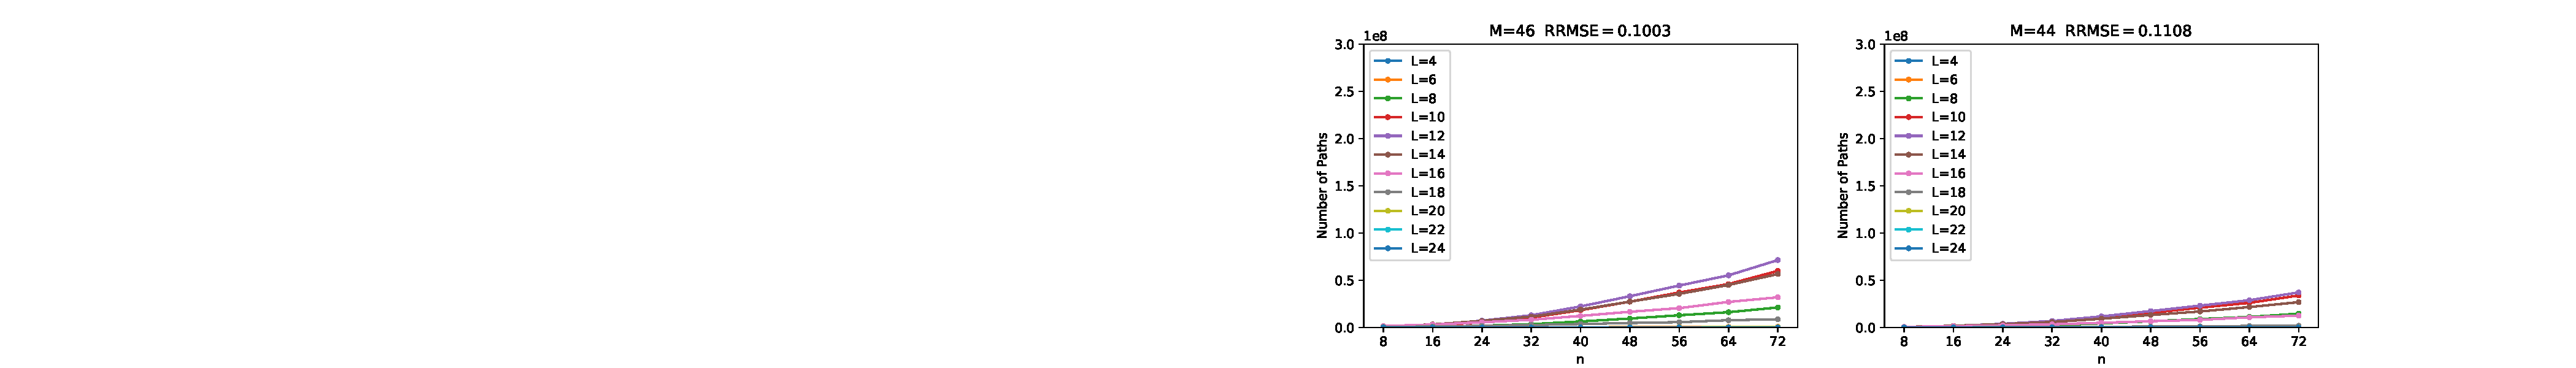
\includegraphics[width=\textwidth]{figures/depth_path2_p2}
    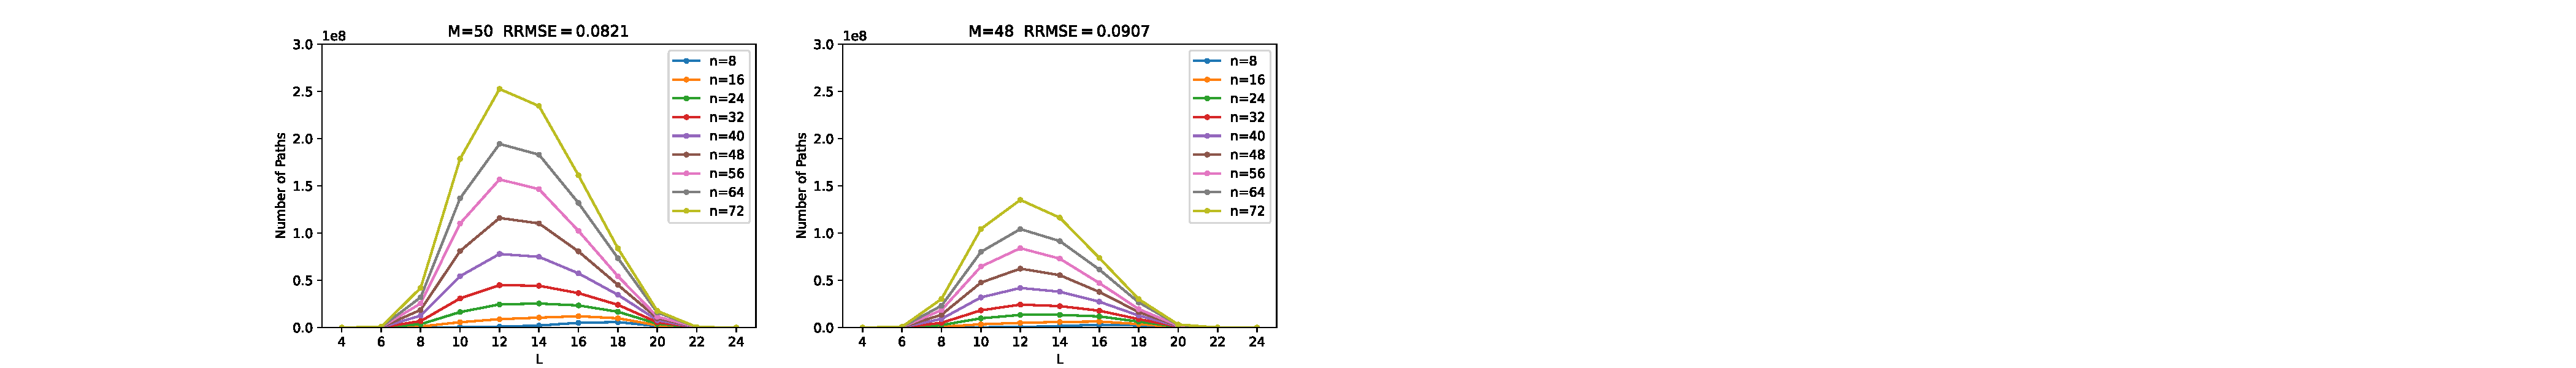
\includegraphics[width=\textwidth]{figures/depth_path_p1}
    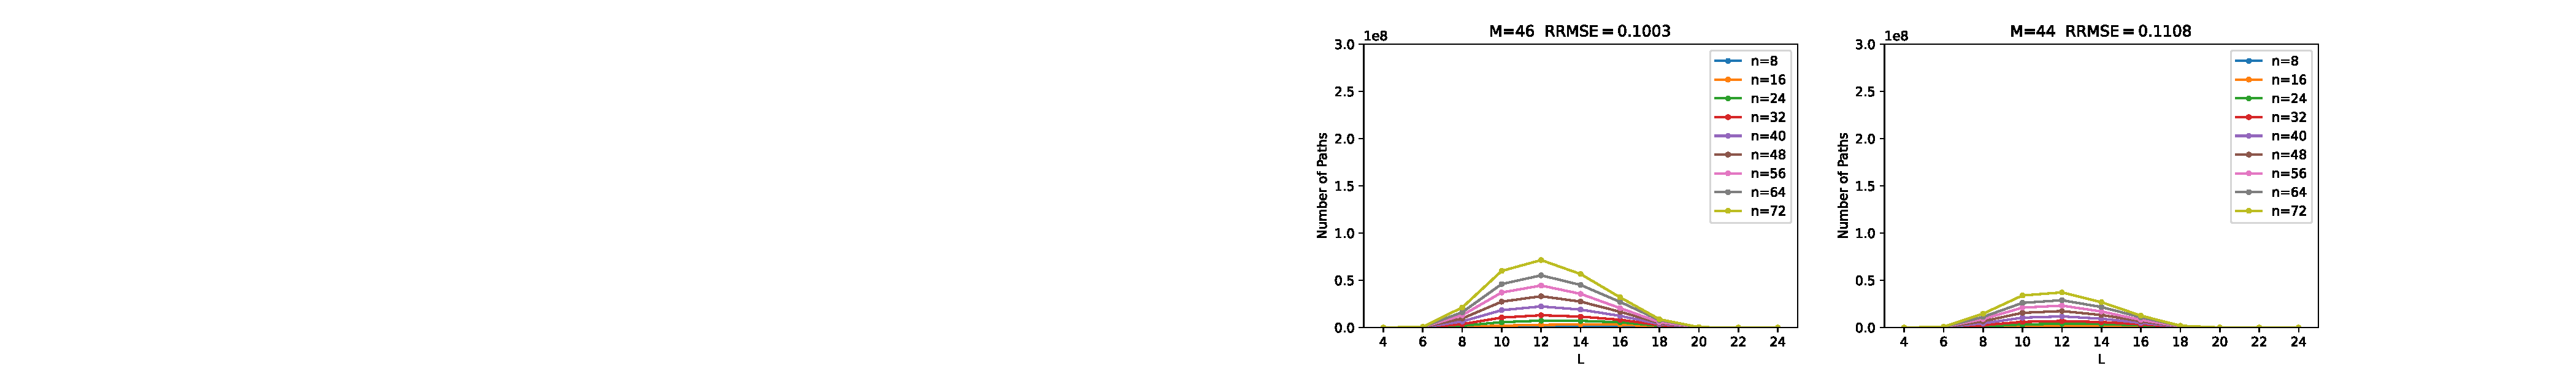
\includegraphics[width=\textwidth]{figures/depth_path_p2}
    \caption{具有非零贡献且$\abs{\bm{s}}\leq M$的Pauli路径$\bm{s}$的数量}\label{fig:numerical_cost}
\end{figure}

根据式~\eqref{eq:depolarizing_M},对于固定的量子线路,不同的截断参数$M$对应于在固定噪声率下由$\frac{\sqrt{\mathbb{E}_{\bm{\theta}}\abs{\widetilde{\langle O \rangle}-\widehat{\langle O \rangle}}^2}}{\norm{O}_\infty}$给出的相对均方根误差界(Relative Root Mean Square Error,RRMSE)。

对于不同的量子比特数$n$和线路的深度$L$,我们计算了权重$\abs{s}\leq M$且具有非零贡献的Pauli路径$s$的数量,结果如图~\ref{fig:numerical_cost}所示。前两行的每个图显示了在固定$M$的情况下,随着$n$的增加,具有非零贡献的Pauli路径的数量的变化。可以看到,在固定$M$的情况下,随着$n$的增加,对所有不同深度$L$的情况,具有非零贡献的Pauli路径的数量将适度增加,并显著小于理论分析的上界$\mathrm{Poly}(n)2^M$。


后两行的每个图显示了在固定$M$的情况下,随着$L$的增加,具有非零贡献的Pauli路径的数量的变化。我们观察到,对于给定的RRMSE界,路径数量先增加然后随着$L$的增加而减少。
这意味着,在给定精度下模拟含噪声量子线路的计算复杂度随着线路深度的增加呈现出先增加后减少的趋势。这与文献~\cite{noh2020efficient}中的发现一致。
其中的RRMSE界是由式~\eqref{eq:depolarizing_M}在噪声率$\lambda=0.2$下给出的。


另一方面,通过式~\ref{eq:depolarizing_M},可以看到不同的截断参数$M$在给定的RRMSE界下也对应了一个具体的噪声强度$\lambda$。
假设,RRMSE界固定为$0.0821$,按图中给出的数据将$M$取值为$M=50,48,46,44$,此时对应的噪声强度为$\lambda=0.2,0.21,0.22,0.23$(两位有效数字)。
从数值结果中可以看到,对于不同的$M$,在给定线路规模$n$和深度$L$的情况下,具有非零贡献的Pauli路径的数量是不同的。这说明在实际的模拟中,噪声的大小将会显著影响模拟算法的计算复杂度。


\subsection{量子线路规模与截断变量$M$的关系}

在本节中,我们研究了在实现可靠精度的情况下,在不同电路规模下截断数$M$的要求。

与前一节类似,我们也以MaxCut问题对应的可观测量为例,在数值上分析$M$与线路规模之间的关系。
对于给定的量子比特数$n$,我们随机生成一个$n\times n$的邻接$(0,1)$矩阵$A$,其中每个条目为$1$的概率为$0.5$。
可观测量为$O=\sum_{A_{i,j}=1} Z_iZ_j$。
初始状态的密度矩阵设为$\rho=\ketbra{0}{0}^{\otimes n}$。

在这一节的模拟中,考虑的量子线路是硬件高效变分量子线路(Hardware Efficient Ans\"atz)~\cite{kandala2017hardwarea}的一个例子,如图~\ref{fig:HEA_Ansatz}所示。
该线路由一系列单量子比特旋转和纠缠的双量子比特门组成,可以分割为$D$个深度为$4$的线路块,每个模块包含两层层作用在所有量子比特上的单量子比特$R_X$和$R_Z$旋转门,以及两层分别以奇数量子比特为控制位和偶数量子比特为目标位的CNOT门。
值得注意的是,双量子比特门的应用仅限于相邻的量子比特,这一设计适合于当前阶段NISQ设备的硬件限制。
对于给定的重复次数$D$,该硬件高效变分量子线路的深度为$4\times D+2$,参数的数量为$2\times D+2$。



\begin{figure}[htbp]
    \centering
    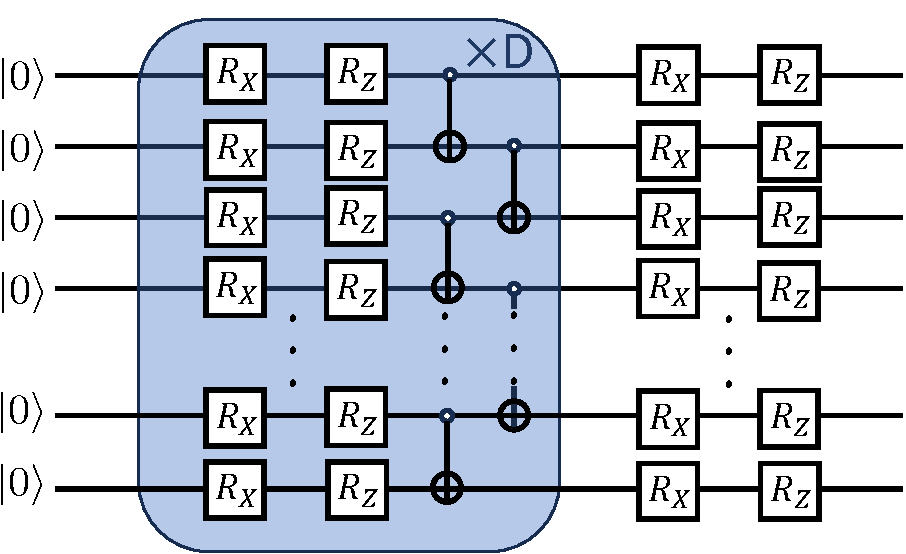
\includegraphics[width=0.5\textwidth]{figures/complexity2/HEA.pdf}
    \caption{Hardware Efficient Ans\"atz}\label{fig:HEA_Ansatz}
\end{figure}

我们随机均匀生成$100$个参数组,记为$\bm{\theta^1}\cdots \bm{\theta^{100}}$,其中每个参数$\bm{\theta^i}$是一个长度为$2\times D+2$的向量,每个元素在$[0,2\pi]$之间均匀分布。
为了方便,记参数取值为参数组$\bm{\theta}$时的含噪声期望值为$\widetilde{\langle O \rangle}(\bm{\theta})$,使用截断数为$M$的Pauli路径积分方法估计的含噪声期望值为$\widehat{\langle O \rangle}(\bm{\theta})$。
我们的数值模拟目标是,找到满足近似含噪声期望值$\widehat{\langle O \rangle}(\bm{\theta})$与精确含噪声期望值$\widetilde{\langle O \rangle}(\bm{\theta})$之间的相对差异在$100$个参数组上均低于$0.1\%$的最小截断数$M$:
\begin{equation}
    \begin{aligned}
        \text{minimize} \quad & M,\\
        \text{subject to} \quad & \widehat{\langle O \rangle}=\sum_{\abs{\bm{s}}\leq M}\tilde{f}(\mathcal{U},\bm{s},O,\rho),\\
        &\max_{i}\frac{\abs{\widetilde{\langle O \rangle}(\bm{\theta^i})-\widehat{\langle O \rangle}(\bm{\theta^i})}}{\abs{\widetilde{\langle O \rangle}(\bm{\theta^i})}}\leq 0.001.
    \end{aligned}
\end{equation}

\begin{figure}[htbp]
    \centering
    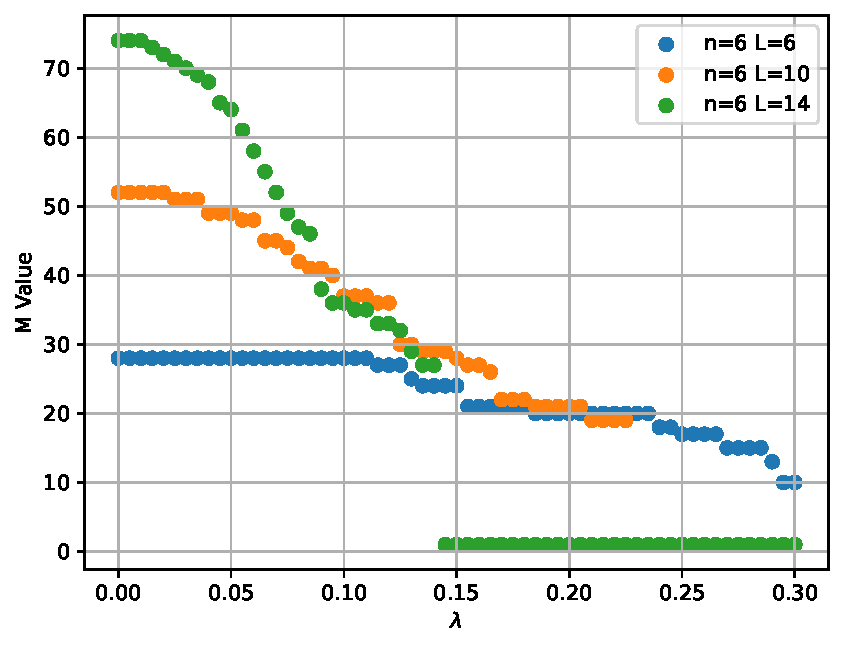
\includegraphics[width=0.45\textwidth]{figures/complexity2/6}
    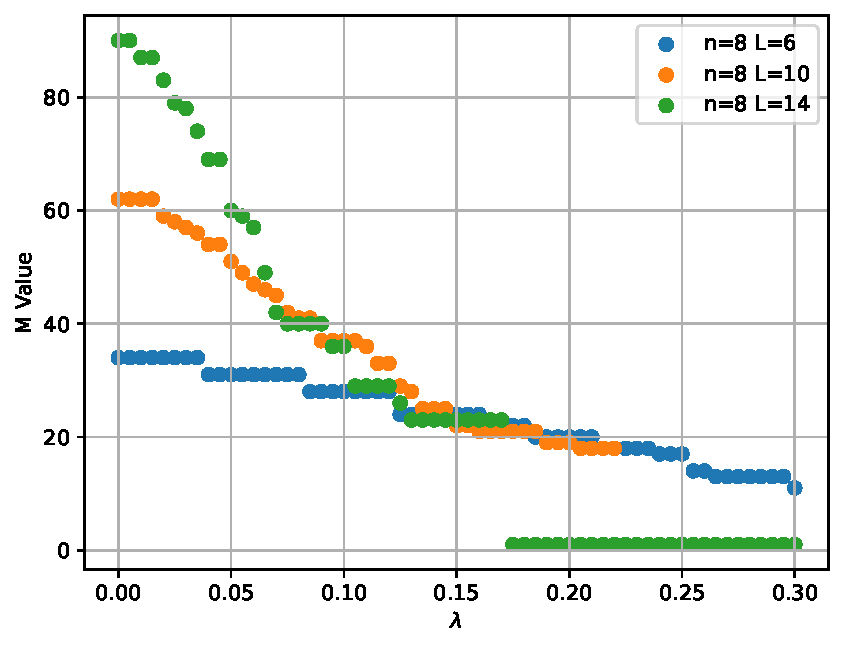
\includegraphics[width=0.45\textwidth]{figures/complexity2/8}
    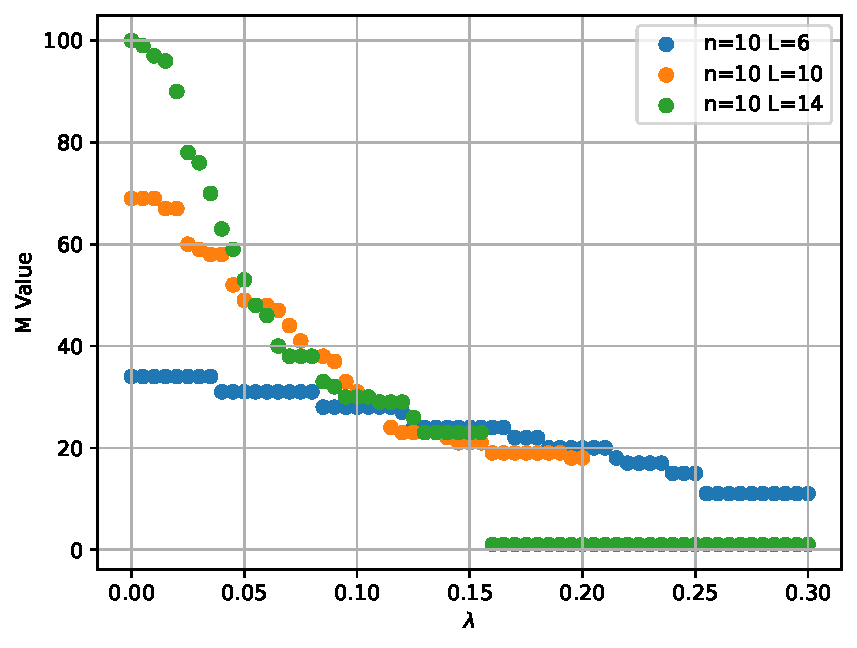
\includegraphics[width=0.45\textwidth]{figures/complexity2/10}
    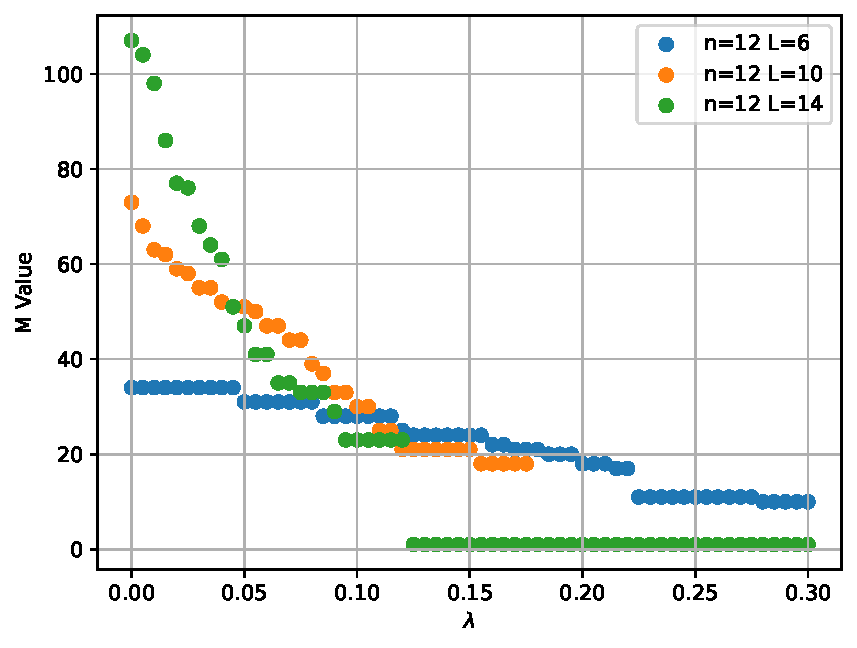
\includegraphics[width=0.45\textwidth]{figures/complexity2/12}
    \caption{满足相对误差要求的最小截断$M$的取值}\label{fig:numerical_M}
\end{figure}

结果如图~\ref{fig:numerical_M}所示。
首先,我们观察到在所有情况下,最小截断$M$随着噪声率$\lambda$的增加而减少。这一趋势与引理~\ref{lemma:MSE_l}中的理论分析一致。
数值结果表明,当噪声率保持在较低水平时,最小截断值$M$随着电路深度$L$线性增加。
这一趋势是由于噪声对Pauli路径的影响较小,导致在浅电路中Pauli路径的传播距离随着电路变深而增加,从而提高了它们的Hamming Weight。因此,在量子线路变深的过程中,为了保留相关的Pauli路径不被丢弃,截断变量$M$需要增加。

当噪声强度较大时,电路深度$L$对于最小截断值$M$的减少速率方面起着关键作用。
这一现象是由于噪声的累积随着电路深度的增加而加剧,导致期望值$\widetilde{\langle O \rangle}(\bm{\theta})$更快地收敛到$\tr{O}$(平凡Pauli路径的贡献)。因此,对于电路深度更深的情况,最小截断值$M$更快地收敛到$0$。

此外,随着量子比特数$n$的增加,最小截断值$M$也趋于增加。
然而,这一增加是适度的,表明OBPPP方法在实际应用中,并不会过度受限于量子比特数$n$的规模。

我们还探讨了在给定电路规模时,精度与截断数$M$之间的关系。当$n = 12$时,我们确定了实现不同精度水平所需的最小$M$值:
\begin{equation}
    \begin{aligned}
        \text{minimize} \quad & M,\\
        \text{subject to} \quad & \widehat{\langle O \rangle}=\sum_{\abs{\bm{s}}\leq M}\tilde{f}(\mathcal{U},\bm{s},O,\rho),\\
        &\max_{i}\frac{\abs{\widetilde{\langle O \rangle}(\bm{\theta^i})-\widehat{\langle O \rangle}(\bm{\theta^i})}}{\abs{\widetilde{\langle O \rangle}(\bm{\theta^i})}}\leq 0.1,0.05,0.01,0.001,0.0001,0.00001,
    \end{aligned}
\end{equation}
分别对应于$90\%,95\%,99\%,99.9\%,99.99\%,99.999\%$的精度。
结果如图~\ref{fig:numerical_ACC}所示,表明所需的最小截断值$M$随着所需精度的增加而增加。


\begin{figure}[htbp]
    \centering
    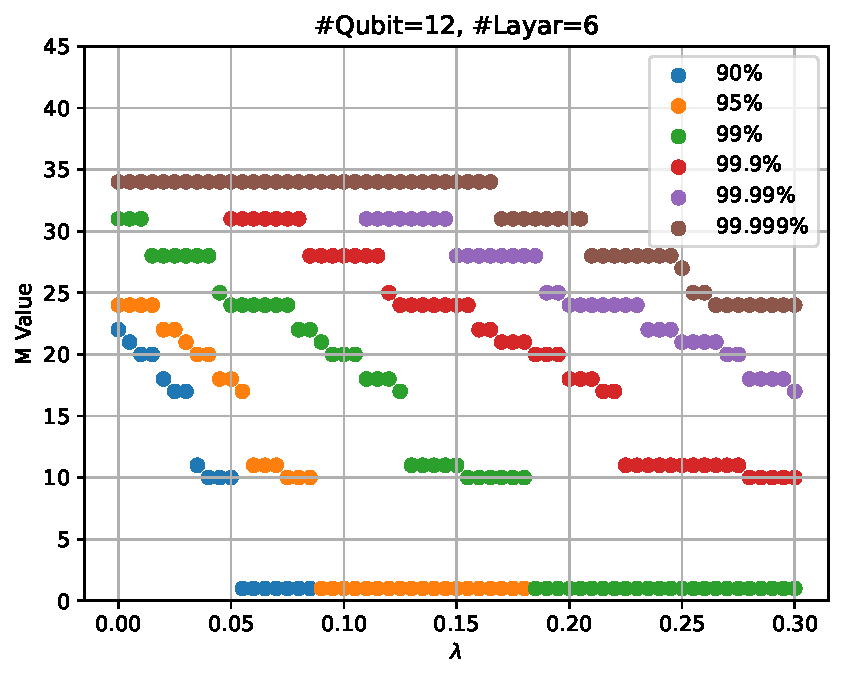
\includegraphics[width=0.32\textwidth]{figures/complexity2/ACC1}
    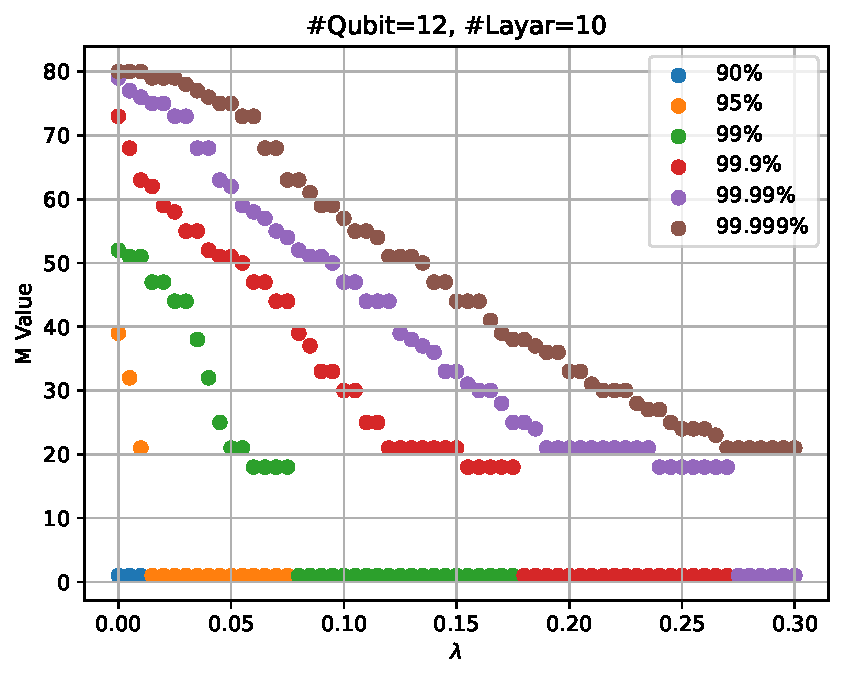
\includegraphics[width=0.32\textwidth]{figures/complexity2/ACC2}
    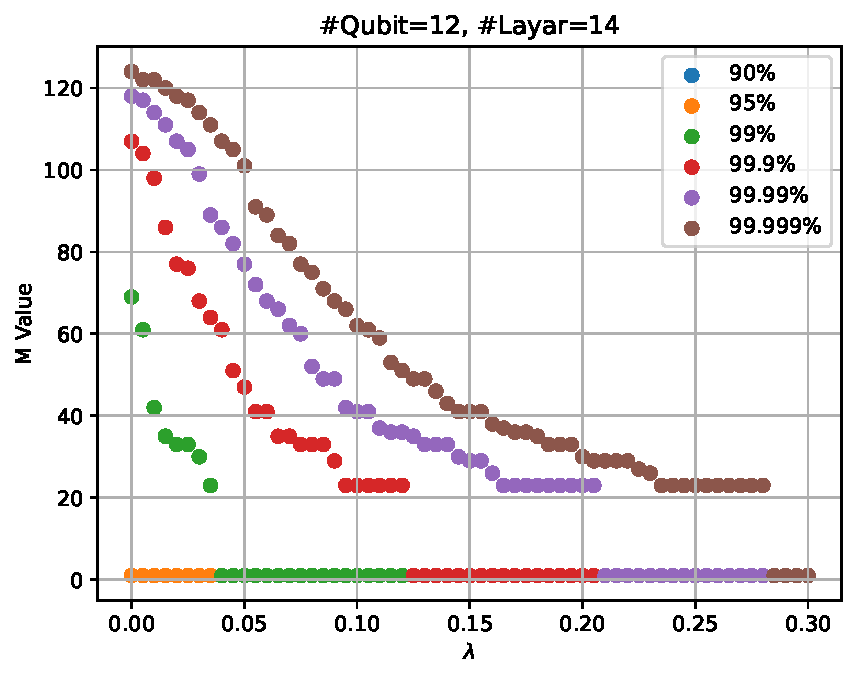
\includegraphics[width=0.32\textwidth]{figures/complexity2/ACC3}
    \caption{
        不同精度水平下所需的最小截断值$M$}\label{fig:numerical_ACC}
\end{figure}

从数值结果可以看出,当对精度的需求迅速增加时,对$M$的需求增加相对温和。
在$L=6$且噪声率$\lambda<0.05$的情况下,实现$>99.9\%$精度所需的最小$M$约为$34$。注意,图中显示的$99.9\%$和$99.99\%$精度对应的结果被$99.999\%$的结果所掩盖。
当噪声率$\lambda$接近$0$时,实现高精度($\geq 99.9\%$)所需的$M$值趋于相同,表明此时$M$足够大以涵盖计算中的足够多的Pauli路径。

当噪声率$\lambda$增加时,实现低精度所需的$M$将比实现高精度所需的$M$减少得更快,这一趋势与引理~\ref{lemma:MSE_l}一致。

对于实现$99.9\%$精度所需的最小截断值$M$,我们通过以下公式估计取定该$M$值时经验均方误差$\tilde{\nu}$:
\begin{equation}\label{ap:eq:emse}
    \tilde{\nu} = \frac{1}{100}\sum_{i=1}^{100}\left|\widetilde{\langle O \rangle}(\bm{\theta^i}) - \widehat{\langle O \rangle}(\bm{\theta^i})\right|^2,
\end{equation}
其中
\begin{equation}
    \begin{aligned}
        \widehat{\langle O \rangle}=&\sum_{\abs{\bm{s}}\leq M}\tilde{f}(\mathcal{U},\bm{s},O,\rho),\\
        M=&\arg\min_{M} \left\{ \max_{i} \frac{\left|\widetilde{\langle O \rangle}(\bm{\theta^i}) - \widehat{\langle O \rangle}(\bm{\theta^i})\right|}{\left|\widetilde{\langle O \rangle}(\bm{\theta^i})\right|} \leq 0.001 \right\}.
    \end{aligned}
\end{equation}
然后将$M$与由式~\ref{eq:depolarizing_M}给出的关于$M$解析界进行比较:
\begin{equation}\label{ap:eq:analytical_bound}
  \frac{1}{2\lambda}\ln{\frac{\norm{O}_\infty^2}{\tilde{\nu}}}.
\end{equation}

\begin{figure}[htbp]
    \centering
    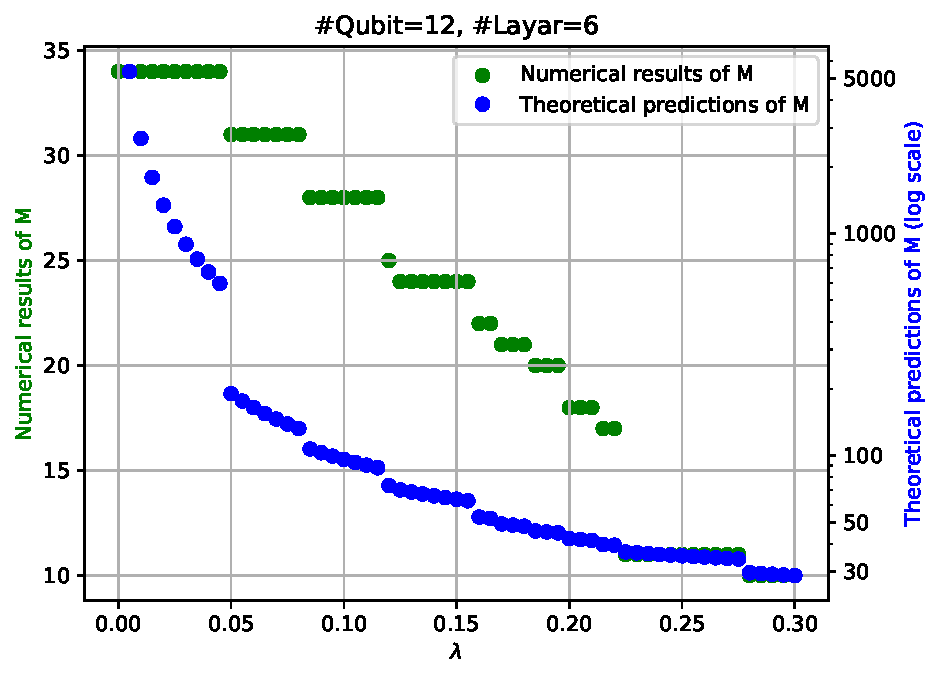
\includegraphics[width=0.32\textwidth]{figures/complexity2/12_1}
    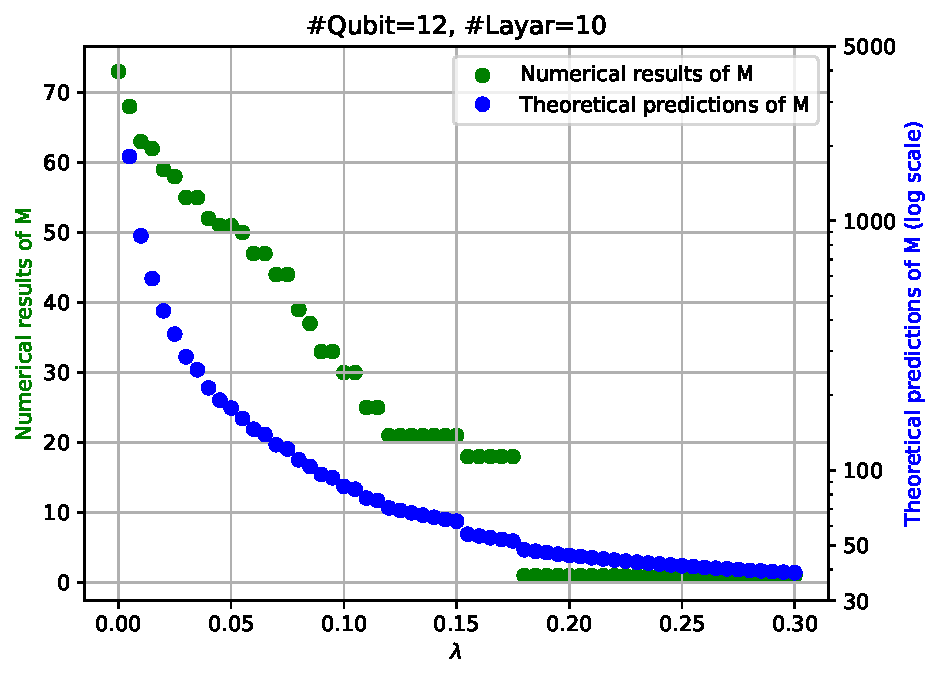
\includegraphics[width=0.32\textwidth]{figures/complexity2/12_2}
    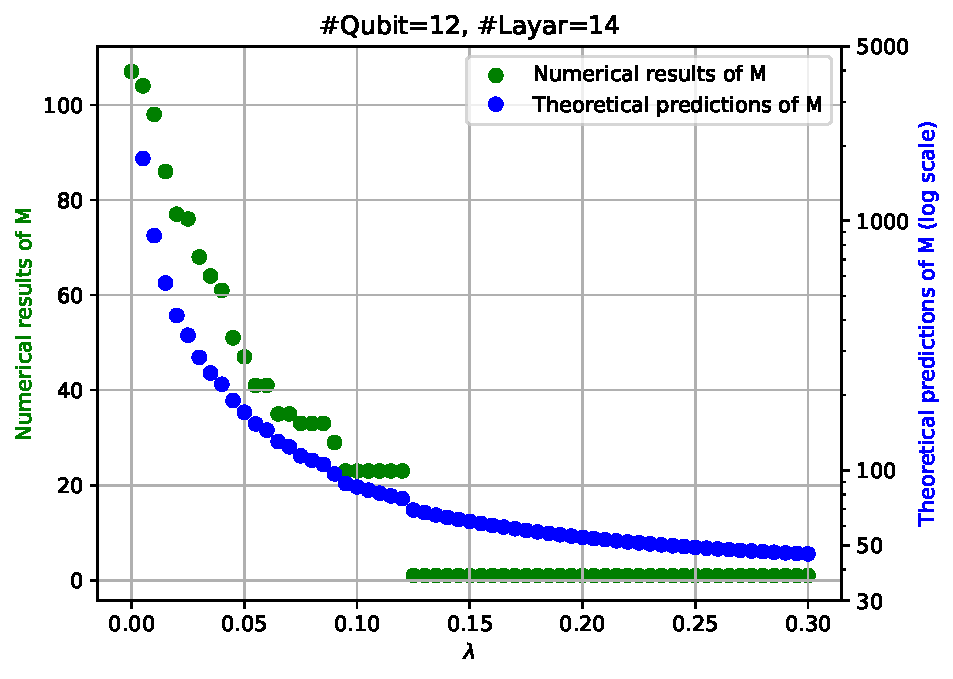
\includegraphics[width=0.32\textwidth]{figures/complexity2/12_3}
    \caption{
        实际应用中所需的最小截断数$M$与理论解析估计的比较}\label{fig:numerical_M2}
\end{figure}

量子比特数$n=12$的对应结果如图~\ref{fig:numerical_M2}所示(其他情况类似)。理论的解析估计结果记为\textit{``Theoretical predictions of M"},为了清晰起见,理论估计的数据使用对数轴显示在右侧。
为了避免式~\eqref{ap:eq:analytical_bound}的分母为$0$,移除了$\lambda=0$的解析估计结果。
结果表明,在实际情况下,为达到目标精度所需的$M$值显著低于理论估计的边界($\sim 100$ vs $\sim 5000$)。

最后,我们展示了在不同噪声率$\lambda$下,经验均方误差$\tilde{\nu}$随$M$增加的变化趋势,以显示收敛趋势。对于$n=12$的情况,如图~\ref{fig:numerical_MSE}所示。
y轴表示经验均方误差,由公式~\ref{ap:eq:emse}给出,并以对数刻度显示。
注意,在图\#Layer=6的数据中中,省略了$M=34$的结果,此时均方误差的值降到了$e^{-20}$以下。

\begin{figure}[htbp]
    \centering
    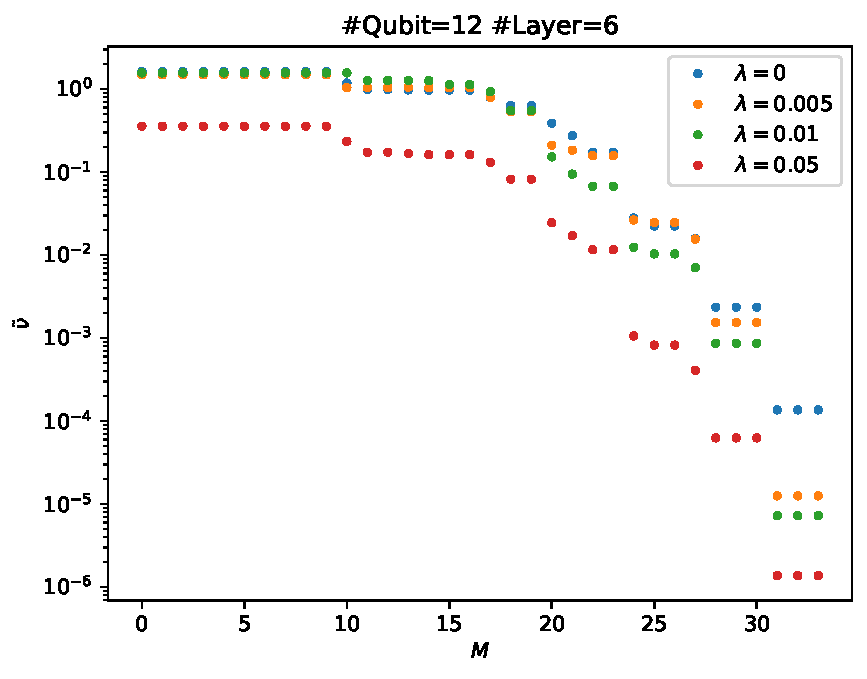
\includegraphics[width=0.32\textwidth]{figures/complexity2/mse_12_6.pdf}
    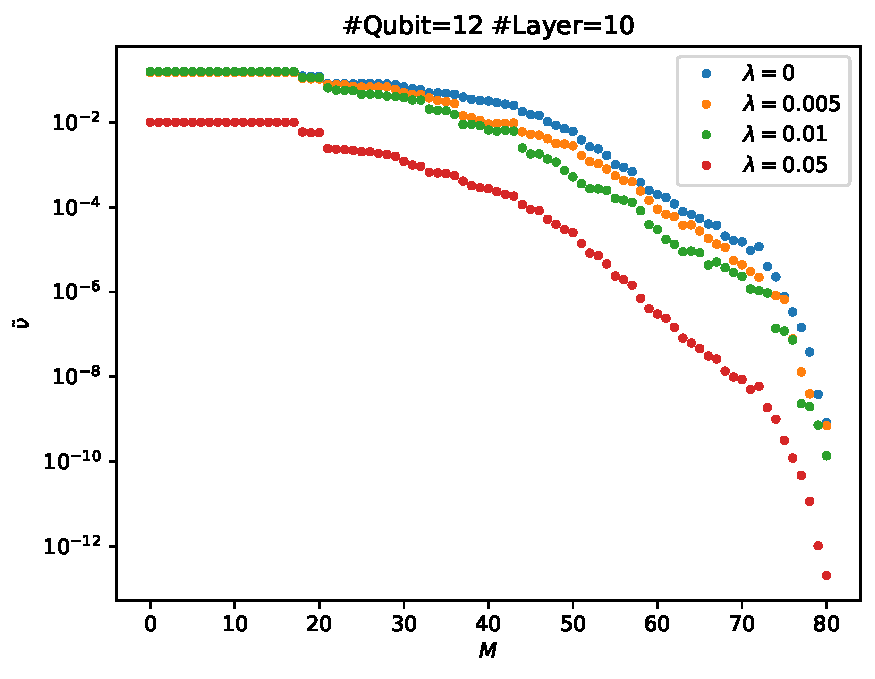
\includegraphics[width=0.32\textwidth]{figures/complexity2/mse_12_10.pdf}
    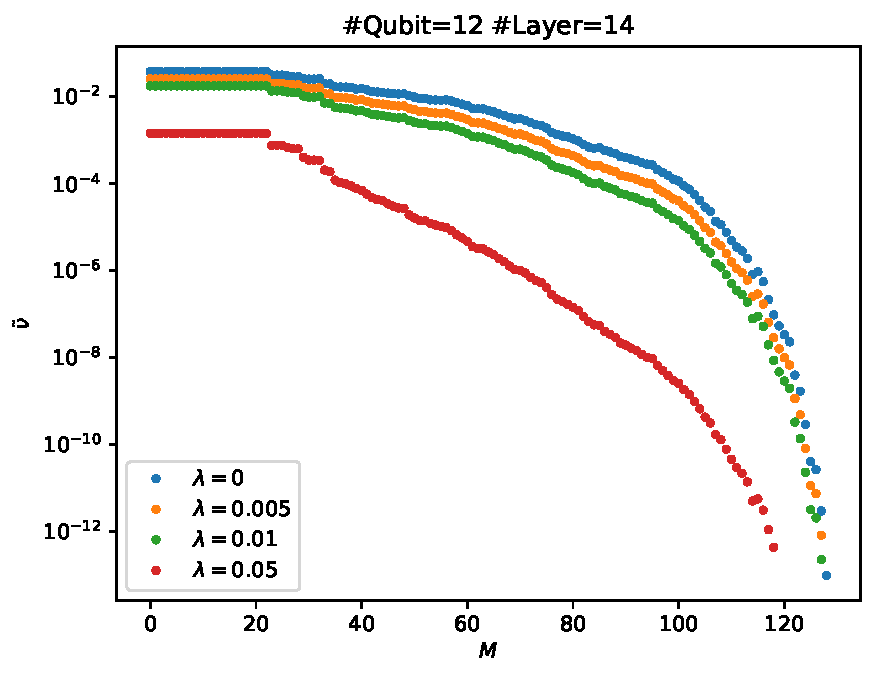
\includegraphics[width=0.32\textwidth]{figures/complexity2/mse_12_14.pdf}
    \caption{对于不同噪声率$\lambda$,$M$增加时的均方误差的变化趋势}\label{fig:numerical_MSE}
\end{figure}


\section{Ising模型演化实验}



在本节中,我们通过对IBM的127量子比特Eagle处理器~\cite{kim2023evidence}进行经典模拟来验证OBPPP方法在实际应用中的效率。
在文献~\cite{kim2023evidence}中,IBM报告了在127量子比特Eagle处理器上的实验,并展示了在一些特定可观测量下期望值的测量。所用的量子线路是由二维横场Ising模型的Trotter时间演化构建的,并被设计为符合Eagle处理器的拓扑结构。
整个量子系统的时间动力学由哈密顿量:
\begin{equation}
  H=-J\sum_{\langle i,j\rangle} Z_iZ_j+h\sum_i X_i,
\end{equation}
控制,其中$J$是耦合强度,$h$是横场强度,$\langle i,j\rangle$表示最近邻的量子比特对。
系统演化过程可以通过哈密顿量的一阶Trotter时间演化来模拟:
\begin{equation}
    \begin{aligned}
        U(\tau)&=\exp{-i\tau H}=\prod_{\langle i,j\rangle} \exp{i\tau J Z_iZ_j}\prod_i \exp{-i\tau h X_i}+\order{\tau^2}\\
        &=\prod_{\langle i,j\rangle}R_{Z_iZ_j}(-2J\tau) \prod_i R_X(2h\tau)+\order{\tau^2},
    \end{aligned}
\end{equation}
其中演化时间$T$被离散化为$N$个Trotter步,每一步的演化时间为$\tau = \frac{T}{N}$。
Trotter时间演化由图~\ref{fig:IBM_Ansatz}所示的量子线路实现,其中一个时间演化步由一层$R_X$门和三层$R_{ZZ}$门组成。
每一步包含一层具有相同旋转角度$\theta_h$的$R_X$门作用于每个量子比特,以及三层具有相同旋转角度$\theta_J$的$R_{ZZ}$门,每层$R_{ZZ}$门作用的量子比特在左侧的Eagle处理器拓扑中显示并用相同颜色标记。
初始状态设为$\rho=\ketbra{0}{0}^{\otimes 127}$。
为了简化,IBM选择$\theta_J=-2J\tau=-\frac{\pi}{2}$,并假设$\theta_h=2h\tau$在$[0,\frac{\pi}{2}]$范围内。
在此模拟中,我们假设硬件中存在退极化噪声$p_x = p_y = p_z = \frac{\lambda}{4}$。

\begin{figure}[htbp]
    \centering
    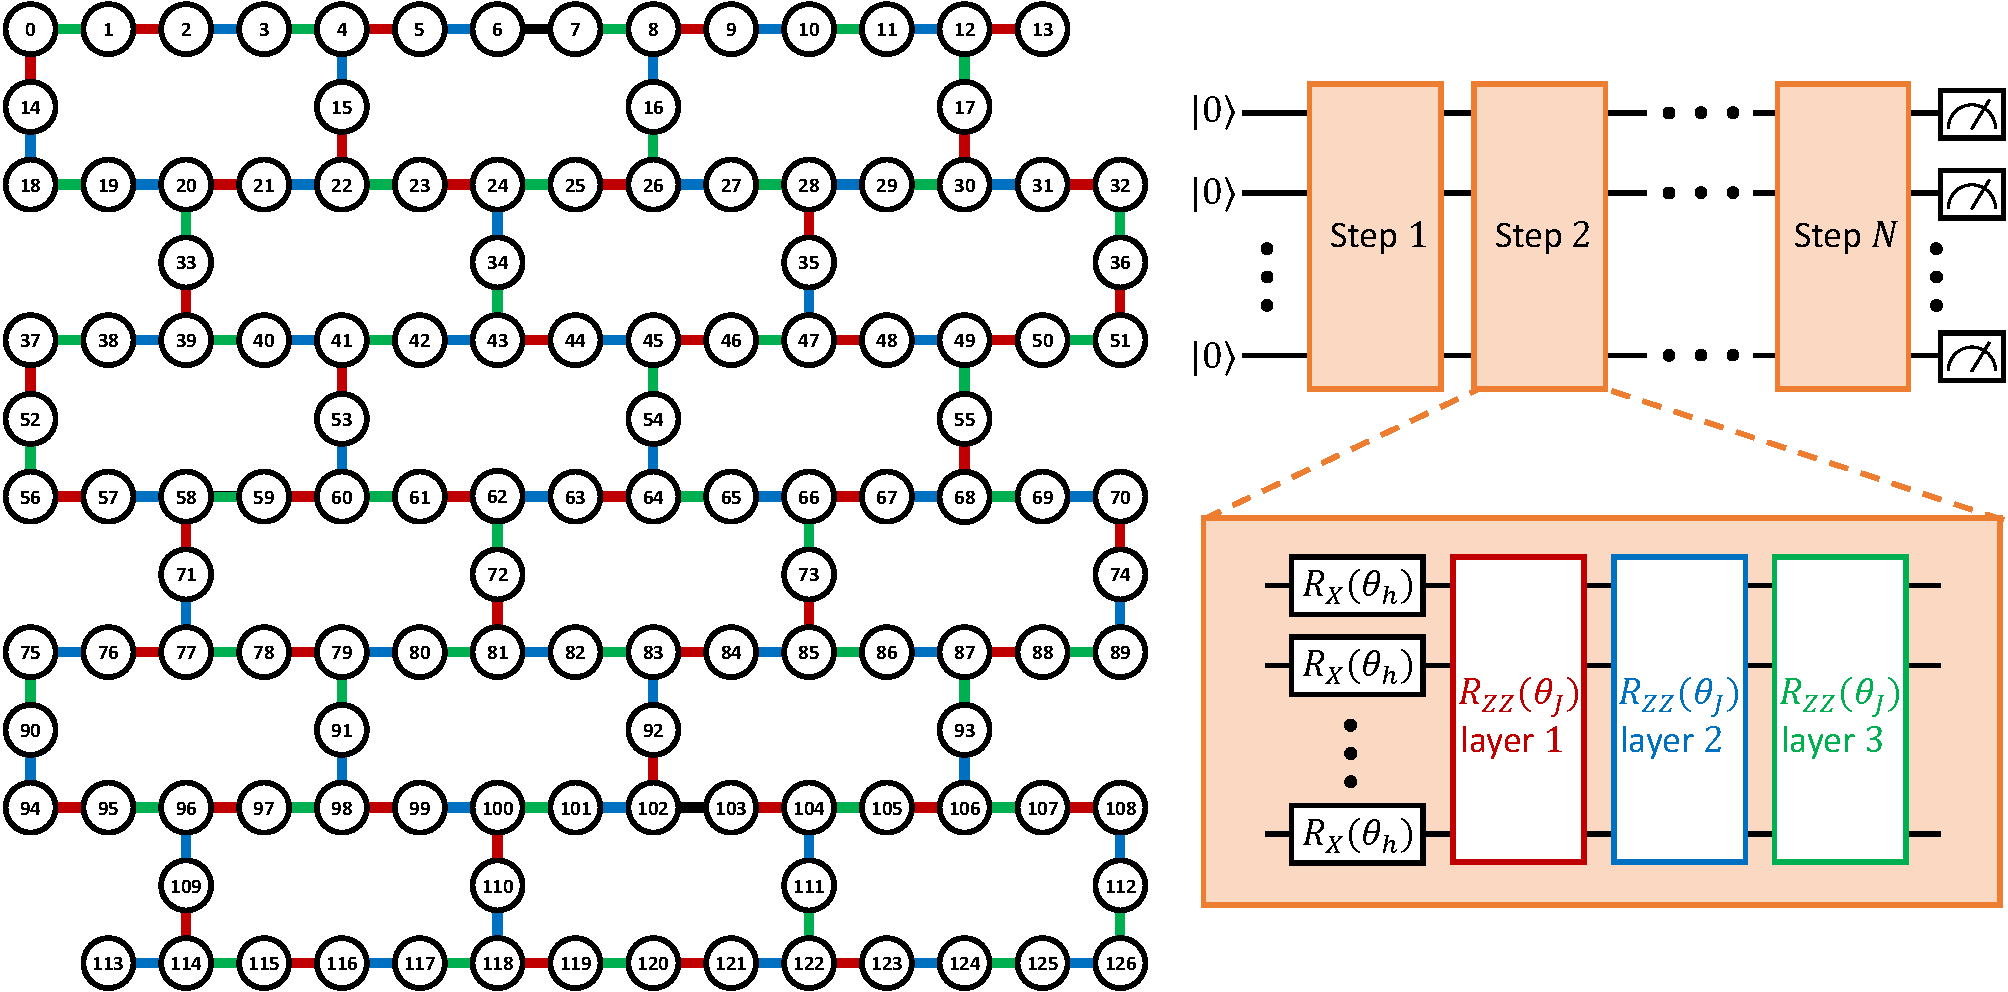
\includegraphics[width=\textwidth]{figures/IBM_Ansatz.pdf}
    \caption{IBM的哈密顿量模拟实验所用的线路}\label{fig:IBM_Ansatz}
\end{figure}

%我们在56核Xeon CPU上使用深度优先搜索策略生成有效路径列表。
在模拟算法的实现中,我们首先使用~\ref{sec:obppp}中描述的反向传播方法找到所有满足条件$\abs{s}\leq M$且具有非零贡献的Pauli路径。随后,我们根据命题~\ref{prop:layer_terms}将这些Pauli路径的贡献函数转换为三角多项式。最后,通过为三角多项式代入不同旋转角度并求和来计算期望值。
值得注意的是,这些Pauli路径贡献实际上表示为$\theta_h$的解析表达式,使我们能够在单次计算中获得整个连续区间内的所有$\theta_h$对应的结果。

使用引理~\ref{lemma:noise},我们可以直接基于贡献的解析表达式计算含噪声量子线路的测量期望值。
这使我们能够直接拟合误差缓解前的原始实验数据。
据我们所知,这是目前唯一能够实现这一目标的经典算法。

%在正文中的图~\ref{fig:IBM}中,我们比较了我们的方法与IBM实验结果在误差缓解(零噪声外推)前后的结果。
为了比较原始实验数据的结果,我们使用经典优化器最小化实验数据集$\{(\theta_h,y_{\theta_h})\}$与我们的近似噪声成本函数$\widehat{\langle O \rangle}$之间的距离,形式化为
\begin{equation}\label{ap:eq:minimal_lambda}
  \lambda=\arg\min_\lambda  \sqrt{\sum_{(\theta_h,y_{\theta_h})\in \mathrm{data set}}\abs{\widehat{\langle O \rangle}(\theta_h)-y_{\theta_h}}^2}.
\end{equation}
在模拟中,我们使用集成在scipy包中的SLSQP优化器来找到$\lambda$~\cite{2020SciPy-NMeth}。


\begin{figure}[htbp]
    \centering
    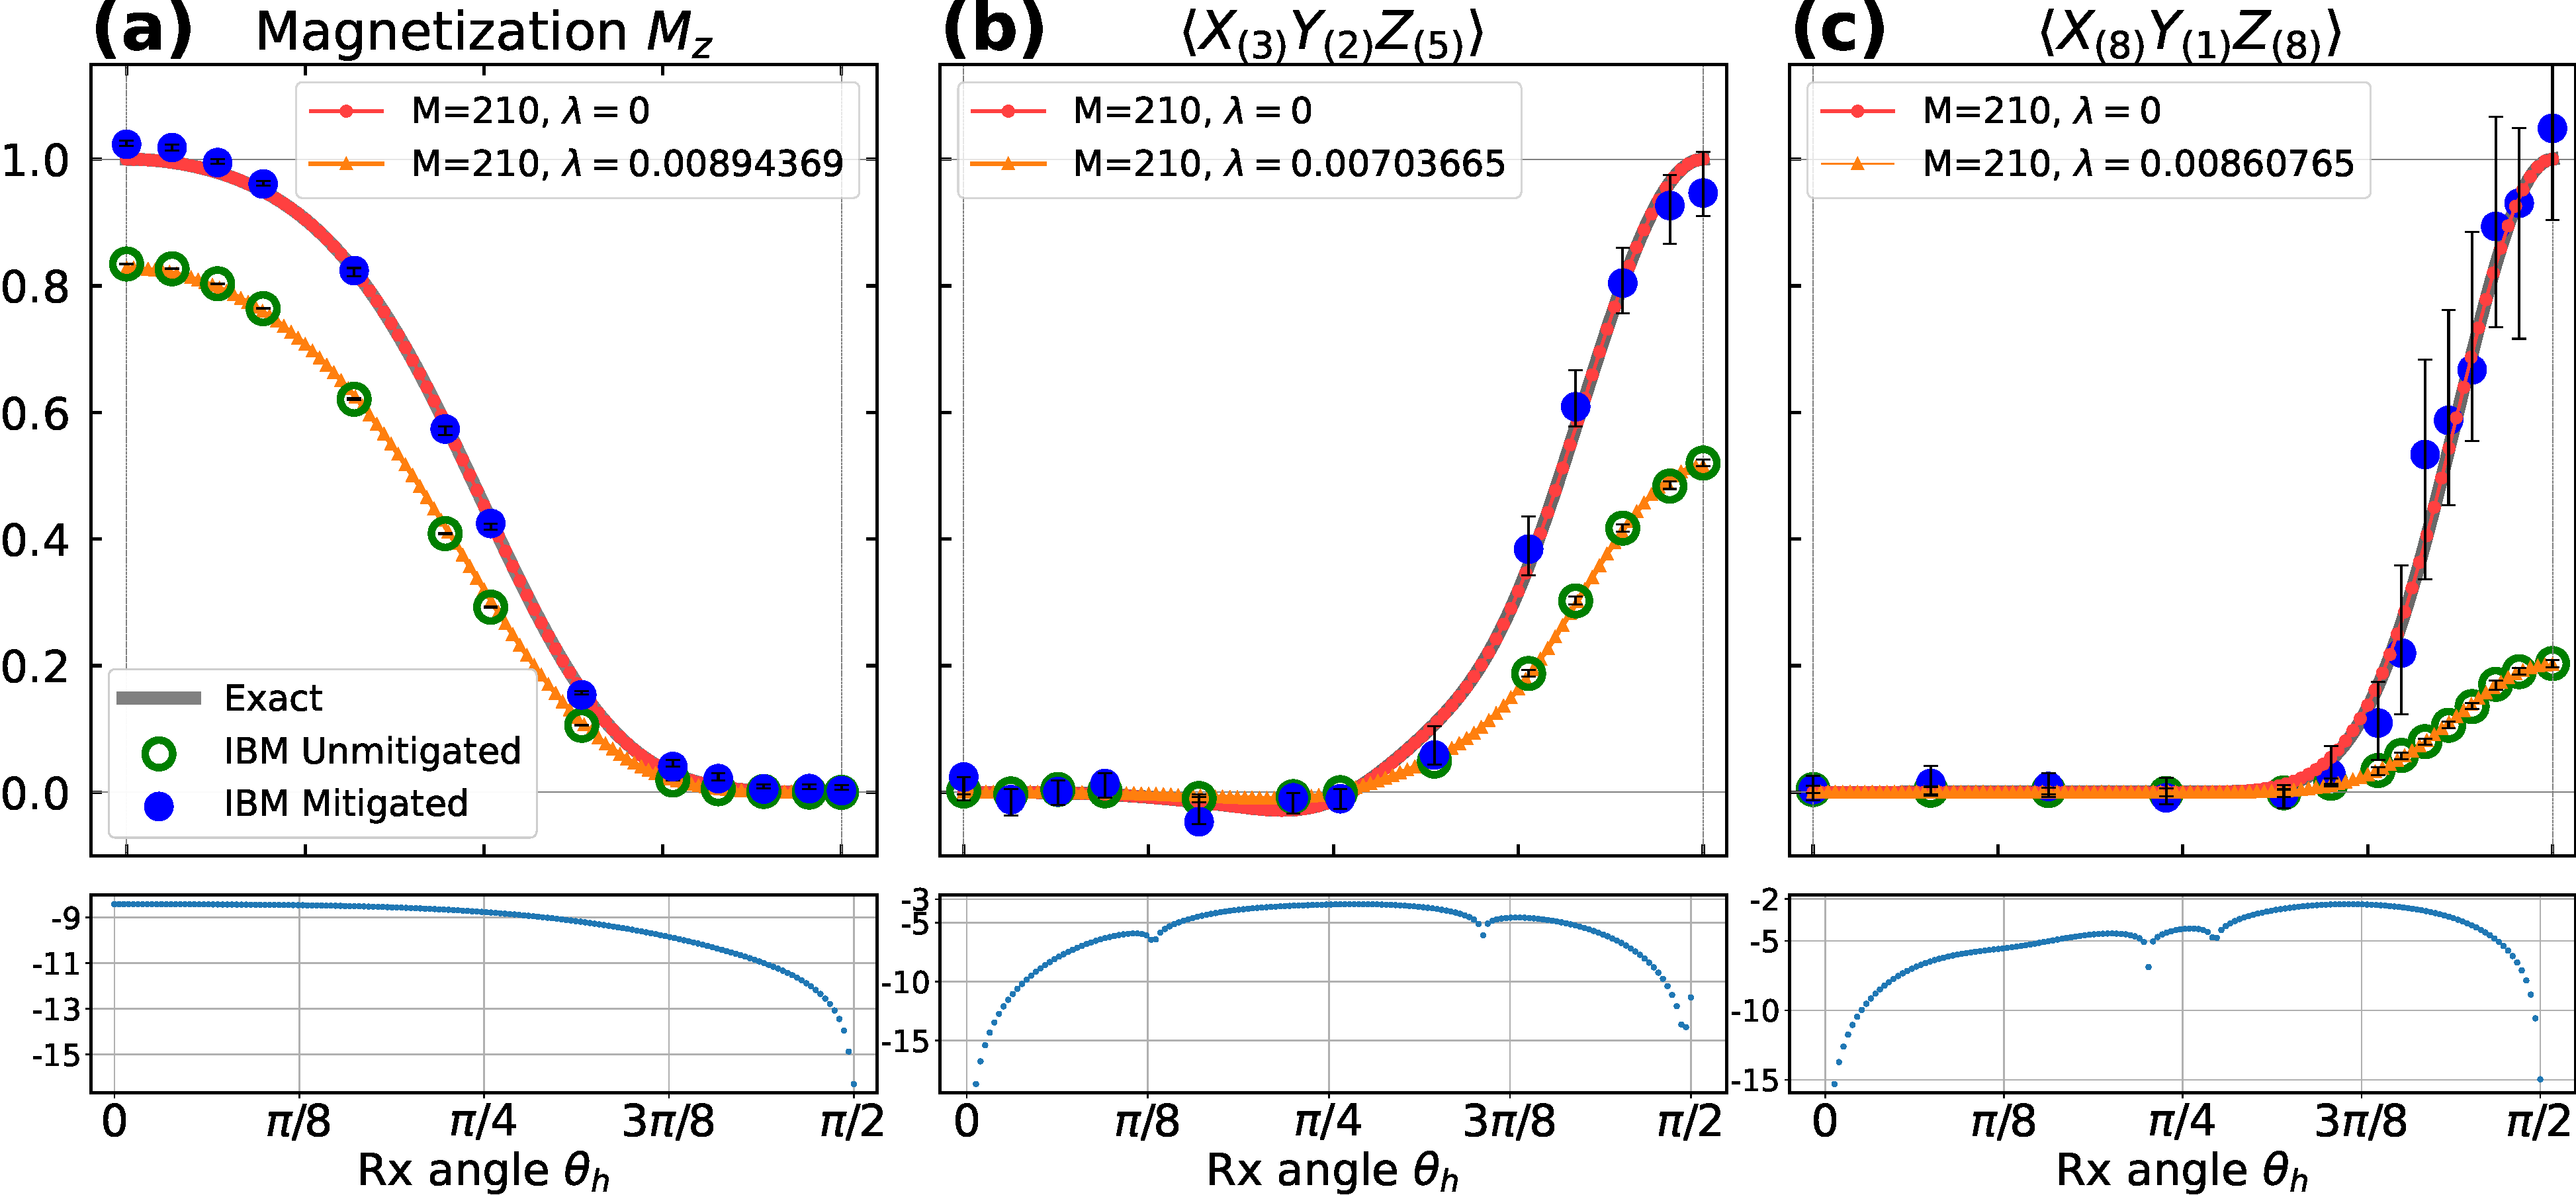
\includegraphics[width=\textwidth]{figures/IBM_F3}
    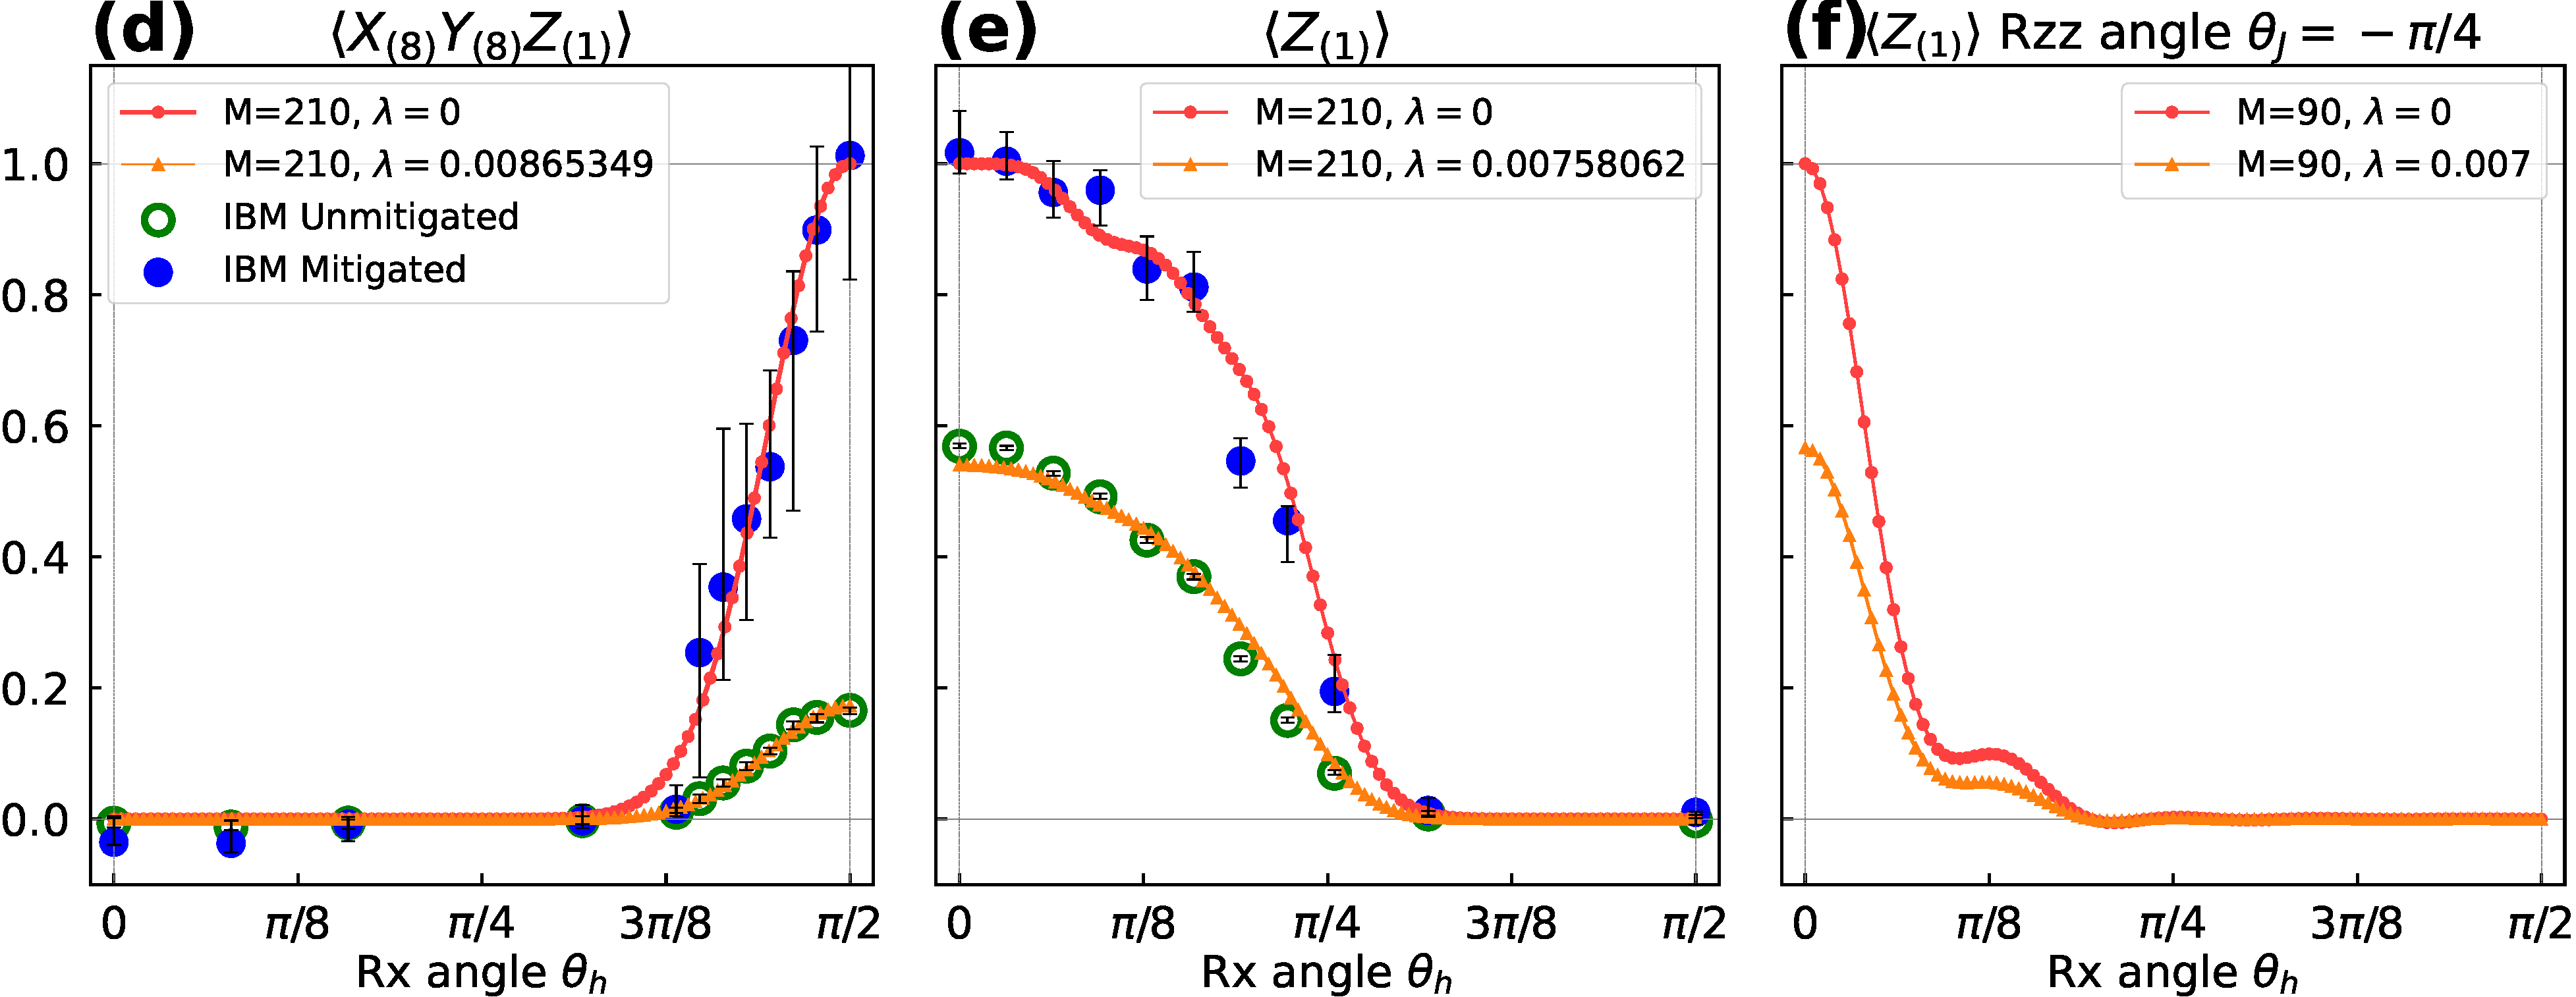
\includegraphics[width=\textwidth]{figures/IBM_F4}
    \caption{IBM的Ising模型演化实验的模拟结果}\label{fig:IBM}
\end{figure}


图~\ref{fig:IBM}展示了IBM在127量子比特Eagle处理器上进行的Ising模型演化实验以及对应的模拟结果。
其中包含了对六种不同实验设定,每种设定的实验量子线路描述如下:
\begin{enumerate}
    \item 在图(a)-(c)中,Trotter步数设为$N=5$,对应于深度为$L=20$的电路。并分别在Hamming Weight 为 $1,10,17$的Pauli算符上进行测量。
    \item 在图(d)中,Trotter步数设为$N=5$,并在电路末尾添加了一层$R_{X}$门,对应于深度为$L=21$的电路。并在Hamming Weight 为 $17$的Pauli算符上进行测量。
    \item 在图(e)中,Trotter步数设为$N=20$,对应于深度为$L=80$的电路。并在Hamming Weight 为 $1$的Pauli算符上进行测量。
    \item 在图(f)中,我们将$R_{ZZ}$门的旋转角设为$\theta_J=-\frac{\pi}{4}$,Trotter步数设为$N=20$,对应于深度为$L=80$的电路。并在Hamming Weight 为 $1$的Pauli算符上进行测量。
\end{enumerate}
图(a)-(e)中的$R_{ZZ}$门的旋转角$\theta_J$设为$\theta_J=-\pi/2$,而(f)中$R_{ZZ}$门的旋转角取自文献~\cite{anand2023classical},设为$\theta_J=-\pi/4$。

图(a)-(e)中的绿色环和蓝色圆分别对应于文献~\cite{kim2023evidence}中报告的不同Pauli算符的直接实验观测结果和经过零噪声推断(Zero-Noise Extrapolation,ZNE)的误差缓解结果。
图(a)-(c)的底部子图显示了OBPPP模拟结果与文献~\cite{kim2023evidence}中呈现的理想精确结果之间的绝对差异。
在每个图中,红点线表示OBPPP模拟的无噪声输出,是关于$\theta_h$三角多项式的解析表达式。
橙色三角线表示在某些噪声抑制下使用截断路径积分近似的含噪声测量期望值。
图(a)-(f)在两颗Xeon 6330 CPU(每颗芯片28核)上的运行时间分别在13秒、146秒、29秒、137秒、262秒和57秒以内。

图(a)-(e)的设定来自文献~\cite{kim2023evidence},(f)的设定来自文献~\cite{anand2023classical}。对于(a)-(c),无噪声理想结果存在精确解,我们发现OBPPP模拟算法(M=210)输出的结果在精度和速度上均优于量子设备~\cite{beguvsic2023fast, kim2023evidence}。
对于(d)-(e),暂时无法获得精确解,所以难以比较无噪声的理想测量期望值,但是可以看到OBPPP的输出结果与IBM的缓解结果非常接近。
在(f)的设定下,暂时缺乏精确结果和实验结果作为比较。
对于(a)-(e),我们使用最小二乘法优化噪声率($p_x=p_y=p_z=\frac{\lambda}{4}$),以拟合噪声电路的期望值。可以看到OBPPP的含噪声期望值模拟结果与IBM未缓解结果之间的强一致性,平均偏差在图(a)-(d)中低于$0.002$,在(e)中均低于$0.008$。优化后的噪声率$\lambda$的范围处于$0.007$到$0.009$,也与IBM报告的误差率一致。



与其他最近的经典模拟算法~\cite{tindall2023efficient,beguvsic2023fast}相比,我们的方法具有两个主要优势:能够获得$\theta_h$的解析表达式,并能够推断含噪声量子线路电路的测量期望值。与张量网络方法~\cite{tindall2023efficient}相比,OBPPP在(b)和(c)中表现出更高的准确性。
在(a)-(e)的所有情况下,OBPPP还表现出更快的执行时间,特别是在更深的电路中~\cite{tindall2023efficient}。
此外,一个显著的区别是,OBPPP在计算(f)时,受到角度变更$\theta_J=\frac{-\pi}{4}$的影响较小。


模拟过程的更多信息和运行时间如表~\ref{tab:IBM}所示:
\begin{table}[h!]
  \centering
  \scalebox{0.6}{
\begin{tabular}{|c|c|c|c|c|c|c|c|c|}
  \hline
    图 & 量子比特数 & 可观测量 & Trotter步数 & 电路深度 & M & 运行时间(56核)&$\min_\lambda  \sqrt{\sum\abs{\widetilde{\langle O \rangle}(\theta_h)-y_{\theta_h}}^2}/\text{\# 数据集}$\\
  \hline
  (a) &127& $M_Z=\sum_q Z_q/n$ &5 & 20 & 210  & 13s&0.0015892257500055675\\
  \hline
  (b) &127& $X_{13,29, 31}Y_{9, 30}Z_{8, 12, 17, 28, 32}$ & 5& 20 & 210  & 146s&0.001395021411390668\\
  \hline
  (c) &127& $X_{37, 41, 52, 56, 57, 58, 62, 79}Y_{75}Z_{38, 40, 42, 63, 72, 80, 90, 91}$ & 5& 20 & 210  & 29s&0.0007674113478406952\\
  \hline
  (d) &127& $X_{37, 41, 52, 56, 57, 58, 62, 79}Y_{38, 40, 42, 63, 72, 80, 90, 91}Z_{75}$ &5& 21 & 210  & 137s&0.0018301118556860437\\
  \hline
  (e) &127& $Z_{63}$ &20& 80 & 210  & 262s&0.007527499236555272\\
  \hline
  (f) &127& $Z_{63}$ &20& 80,$\theta_J=-\pi/4$ & 90  & 57s&\\
  \hline
\end{tabular}}
\caption{IBM的Ising模型演化任务的比较和经典模拟的运行时间}\label{tab:IBM}
\end{table}


\section{QAOA算法实验}


    在上一节中,我们进行了IBM的Ising模型演化实验的模拟,IBM的实验运行一个典型的超导量子比特系统中。
    在本节中,我们将模拟文献~\cite{pagano2020quantum}中报告的离子阱系统的实验结果,并得到高度一致的结果。
    
    在实验中,作者使用了一维排列的$^{171}$Yb$^+$离子,并使用该离子系统实现了低深度长程的量子近似优化算法(QAOA)的演示实验。
    在该QAOA算法中,优化问题被编码在具有长程相互作用的横场反铁磁Ising模型哈密顿量中:
    \begin{equation}\label{eq:qaoa:hamiltonian}
        H=\underbrace{\sum_{i<j}J_{ij}X_iX_j}_{H_A}+\underbrace{B\sum_iY_i}_{H_B}.
    \end{equation}
    其中,$J_{i,j}>0$表示自旋$i$和$j$之间的Ising耦合强度,随自旋间距离按幂律衰减;$B$表示横向磁场强度。为了方便我们将$\sum_{i<j}J_{ij}X_iX_j$记为$H_A$,$B\sum_iY_i$记为$H_B$。
    
    系统的初态度经过$p$层QAOA线路块演化后的状态为:
    \begin{equation}
      \ket{\vec{\beta},\vec{\gamma}}=\prod_{k=1}^p e^{-i\beta_k (H_B/J_0)} e^{-i\gamma_k (H_A/J_0)}\ket{\psi_0},
    \end{equation}
    其中$J_0$是最近邻耦合的平均值,角度向量$\vec{\beta}$和$\vec{\gamma}$是用于最小化最终能量的变分参数:
    \begin{equation}
      E(\vec{\beta},\vec{\gamma})=\bra{\vec{\beta},\vec{\gamma}}H\ket{\vec{\beta},\vec{\gamma}}。
    \end{equation}
    初始状态设为$\ket{\psi_0}=\ket{\uparrow\uparrow\dots\uparrow}_Y$,其中$\ket{\uparrow}_Y=(\ket{\uparrow}_Z+i\ket{\downarrow}_Z)/\sqrt{2}$。
    
    在原实验设定中,作者使用无量纲相对量:
    \begin{equation}\label{ap:eq:qaoa:eta}
      \eta=\frac{E(\vec{\beta},\vec{\gamma})-E_{\max}}{E_{gs}-E_{\max}}
    \end{equation}
    来衡量QAOA算法输出结果的表现,其中$E_{gs}$是哈密顿量~\eqref{eq:qaoa:hamiltonian}的基态能量,$E_{\max}$表示最高激发态的能量。
    
    在本节中,我们将使用OBPPP算法模拟文献~\cite{pagano2020quantum}中图2C的实验结果。
    在该实验中,量子比特数为$n=12$,QAOA线路块的层数为$p=1$。
    在我们的模拟过程中,Ising模型的耦合强度$J_{ij}$设为文献~\cite{pagano2020quantum}补充信息中给出的解析拟合形式:
    \begin{equation}
      J_{ij}\approx\frac{J_0}{r^{\alpha^\prime}}e^{-\beta^\prime(r-1)},
    \end{equation}
    其中$J_0$是最近邻耦合的平均值,$r=\abs{i-j}$是离子间距,$\alpha^\prime,\beta^\prime$是指数衰减变量。
    根据参考文献中的设定,$J_0=0.580$,$\alpha^\prime=0.322$,$\beta^\prime=0.229$,横向磁场满足$B/J_0=-0.25$。
    
    \begin{figure}[hbp]	
        \centering
        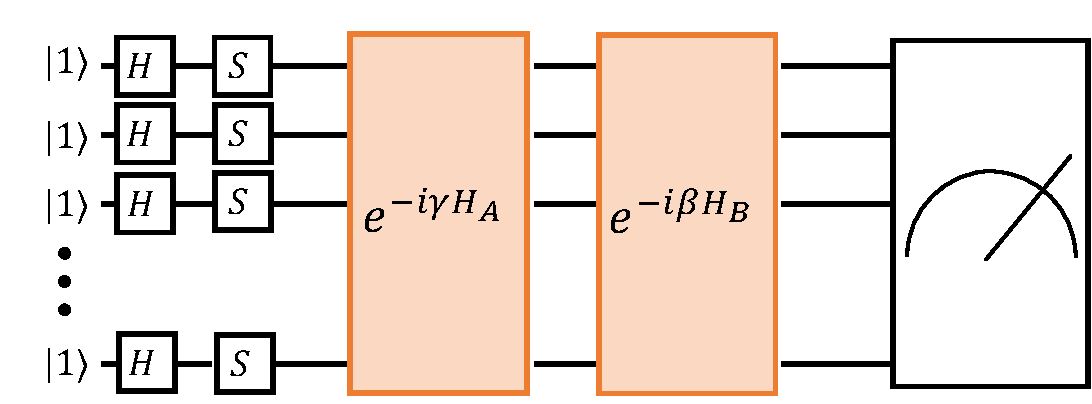
\includegraphics[width=0.75\textwidth]{figures/Ion_ansatz.pdf}
        \caption{QAOA实验模拟中使用的12量子比特电路}\label{fig:Ion_Ansatz}
    \end{figure}
    
    模拟中使用的电路如图~\ref{fig:Ion_Ansatz}所示。通过以下公式:
    \begin{equation}
        SH\ket{1}=S(\ket{0}-\ket{1})/\sqrt{2}=(\ket{0}-i\ket{1})/\sqrt{2}=-i\ket{\uparrow}_Y,
    \end{equation}
    我们使用初始状态$\ket{1}$并通过一层$H$门和一层$S$门,等效生成实验中的初始状态$\ket{\psi_0}$。
    电路中对应于$H_A$部分的演化:
    \begin{equation}
        e^{-i\gamma (H_A/J_0)}=e^{-i\gamma \sum (J_{ij}/J_0)X_iX_j},
    \end{equation}
    可以通过一系列$R_{XX}$门,利用$\Pi e^{-i\gamma(J_{ij}/J_0)X_iX_j}$来实现。
    因为在实验中总共有$(^{12}_2)=66$对相互作用(或$R_{XX}$门),这些$R_{XX}$门可以按最紧凑的排列方式在电路中使用$66/6=11$层线路实现。
    而演化对应于$H_B$的部分$e^{-i\beta (H_B/J_0)}=e^{-i\beta \sum(B/J_0)Y_i}$,可以由一层作用于每个量子比特的$R_Y$门实现。
    %初始状态$\ket{1}$首先通过一层$H$门和一层$S$门,等效生成实验中的初始状态$\ket{\psi_0}$。
    电路中对应于$H_A$的演化由11层不重叠的$R_{XX}$门实现,对应于$H_B$的演化由一层作用于每个量子比特的$R_Y$门实现,而生成初始态制备需要额外的两层线路,于是电路的总层数为14层。
    
    \begin{figure}[htbp]
        \centering
        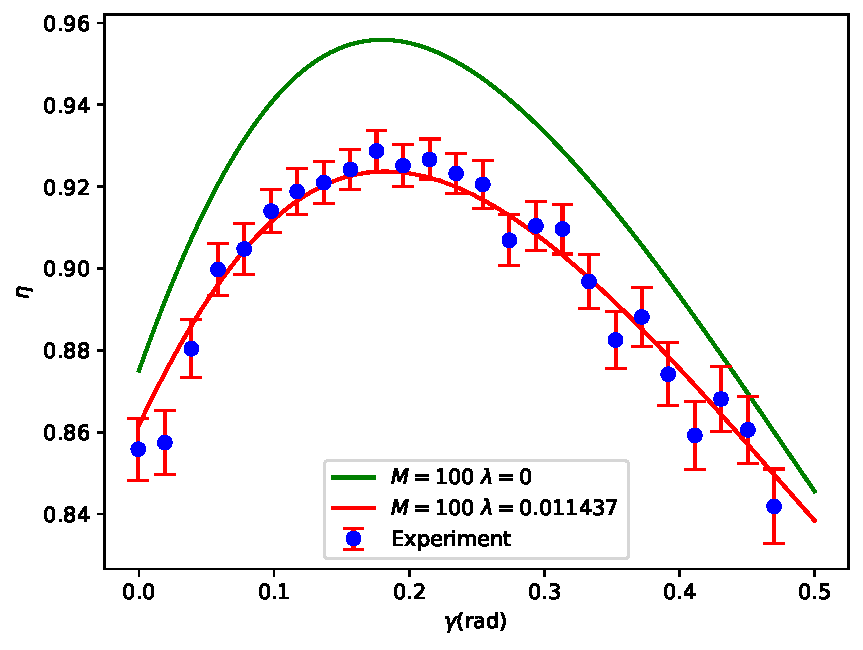
\includegraphics[width=0.95\textwidth]{figures/QAOA.pdf}
        \caption{QAOA实验结果与模拟结果的比较}\label{fig:QAOA_result}
    \end{figure}
    
    在文献~\cite{pagano2020quantum}的图2C中,作者报告了设定角度$\beta^\star=1.12$时,测量期望值视角度$\eta$为变分参数$\gamma$的函数的实验结果。
    模拟结果如图~\ref{fig:QAOA_result}所示,y轴$\eta$定义在式~\ref{ap:eq:qaoa:eta}中。
    为了模拟退极化噪声$p_x = p_y = p_z = \frac{\lambda}{4}$存在时的含噪声测量期望值结果,类似于前一节,我们使用SLSQP优化器优化式~\ref{ap:eq:minimal_lambda}以获得合适的噪声率$\lambda$来拟合实验结果。
    优化后所得的最佳噪声率为$\lambda=0.011437$。
    从图中可以看出,噪声的出现影响了QAOA的性能,实验结果相比于无噪声推测结果略低。
    与实验结果相比较,在这个离子阱系统实验中,我们的方法很好地拟合了含噪声的实验结果,表明OBPPP方法在实际应用中具有很好的适用性。